\documentclass[a4paper]{article} 
\addtolength{\hoffset}{-2.25cm}
\addtolength{\textwidth}{4.5cm}
\addtolength{\voffset}{-3.25cm}
\addtolength{\textheight}{5cm}
\setlength{\parskip}{0pt}
\setlength{\parindent}{0in}

%----------------------------------------------------------------------------------------
%	PACKAGES AND OTHER DOCUMENT CONFIGURATIONS
%----------------------------------------------------------------------------------------

\usepackage{blindtext} % Package to generate dummy text
\usepackage{charter} % Use the Charter font
\usepackage[utf8]{inputenc} % Use UTF-8 encoding
\usepackage{microtype} % Slightly tweak font spacing for aesthetics
\usepackage[english]{babel} % Language hyphenation and typographical rules
\usepackage{amsthm, amsmath, amssymb} % Mathematical typesetting
\usepackage{float} % Improved interface for floating objects
\usepackage[final, colorlinks = true, 
            linkcolor = black, 
            citecolor = black]{hyperref} % For hyperlinks in the PDF
\usepackage{graphicx, multicol} % Enhanced support for graphics
\usepackage{xcolor} % Driver-independent color extensions
\usepackage{marvosym, wasysym} % More symbols
\usepackage{rotating} % Rotation tools
\usepackage{censor} % Facilities for controlling restricted text
\usepackage{listings, style/lstlisting} % Environment for non-formatted code, !uses style file!
\usepackage{pseudocode} % Environment for specifying algorithms in a natural way
\usepackage{style/avm} % Environment for f-structures, !uses style file!
\usepackage{booktabs} % Enhances quality of tables
\usepackage{tikz-qtree} % Easy tree drawing tool
\tikzset{every tree node/.style={align=center,anchor=north},
         level distance=2cm} % Configuration for q-trees
\usepackage{style/btree} % Configuration for b-trees and b+-trees, !uses style file!
\usepackage{csquotes} % Context sensitive quotation facilities
\usepackage[yyyymmdd]{datetime} % Uses YEAR-MONTH-DAY format for dates
\renewcommand{\dateseparator}{-} % Sets dateseparator to '-'
\usepackage{fancyhdr} % Headers and footers
\pagestyle{fancy} % All pages have headers and footers
\fancyhead{}\renewcommand{\headrulewidth}{0pt} % Blank out the default header
\fancyfoot[L]{} % Custom footer text
\fancyfoot[C]{} % Custom footer text
\fancyfoot[R]{\thepage} % Custom footer text
\newcommand{\note}[1]{\marginpar{\scriptsize \textcolor{red}{#1}}} % Enables comments in red on margin

%----------------------------------------------------------------------------------------

\begin{document}

%-------------------------------
%	TITLE SECTION
%-------------------------------

\fancyhead[C]{}
\hrule \medskip % Upper rule
\begin{minipage}{0.295\textwidth} 
\raggedright
\footnotesize
Andrew Hayes \hfill\\   
21321503 \hfill\\
a.hayes18@nuigalway.ie
\end{minipage}
\begin{minipage}{0.4\textwidth} 
\centering 
\large 
CT255 Assignment 2\\ 
\normalsize 
Rainbow Tables\\ 
\end{minipage}
\begin{minipage}{0.295\textwidth} 
\raggedleft
\today\hfill\\
\end{minipage}
\medskip\hrule 
\bigskip

%-------------------------------
%	CONTENTS
%-------------------------------

\section{Problem 1}
\subsection{Code}
\begin{lstlisting}[language=Java]
import java.util.HashMap;

/*  CT255 Assignment 2
 *  This class provides functionality to build rainbow tables (with a different reduction function per round) for 8 character long strings, which
    consist of the symbols "a .. z", "A .. Z", "0 .. 9", "!" and "#" (64 symbols in total).
    Properly used, it creates the following value pairs (start value - end value) after 10,000 iterations of hashFunction() and reductionFunction():
          start value  -  end value
          Kermit12        lsXcRAuN
          Modulus!        L2rEsY8h
          Pigtail1        R0NoLf0w
          GalwayNo        9PZjwF5c
          Trumpets        !oeHRZpK
          HelloPat        dkMPG7!U
          pinky##!        eDx58HRq
          01!19!56        vJ90ePjV
          aaaaaaaa        rLtVvpQS
          aaaaaaaa        klQ6IeQJ
          
          
 *
 * @author Michael Schukat
 * @version 1.0
 */
public class RainbowTable
{
    public static void main(String[] args) {
		long res = 0;

        // String array of the known passwords
        String[] passwords = {"Kermit12", "Modulus!", "Pigtail1", "GalwayNo", "Trumpets", "HelloPat", "pinky##!", "01!19!56", "aaaaaaaa", "aaaaaaaa"};

        HashMap<String, String> rainbowTable = new HashMap<>(); // declaring a HashTable that i'll use to store the password : hash pairs


        // looping through the passwords array
		for (String start : passwords) {
            if (start.length() != 8) {
                System.out.println("Input " + start + " must be 8 characters long - Exit");
            }
            else {
                String hash = start;                             // declaring a String hash that will hold the final reduced hash of a given password

                // hashing & reducing the start String 10000 times.
                for (int i = 0; i < 10000; i++) {
                    hash = reductionFunction((hashFunction(hash)), i);
                }

                // adding the password & its hash value to the rainbowTable HashMap
                rainbowTable.put(start, hash);
            }
        }
        // printing out the contents of the rainbowTable
        System.out.println(rainbowTable);
	}
        
    private static long hashFunction(String s){
        long ret = 0;
        int i;
        long[] hashA = new long[]{1, 1, 1, 1};
        
        String filler, sIn;
        
        int DIV = 65536;
        
        filler = new String("ABCDEFGHABCDEFGHABCDEFGHABCDEFGHABCDEFGHABCDEFGHABCDEFGHABCDEFGH");
        
        sIn = s + filler; // Add characters, now have "<input>HABCDEF..."
        sIn = sIn.substring(0, 64); // // Limit string to first 64 characters

        for (i = 0; i < sIn.length(); i++) {
            char byPos = sIn.charAt(i); // get i'th character
            hashA[0] += (byPos * 17111); // Note: A += B means A = A + B
            hashA[1] += (hashA[0] + byPos * 31349);
            hashA[2] += (hashA[1] - byPos * 101302);
            hashA[3] += (byPos * 79001);
        } 
           
        ret = (hashA[0] + hashA[2]) + (hashA[1] * hashA[3]);
        if (ret < 0) ret *= -1;
        return ret;
    } 
    
    private static String reductionFunction(long val, int round) {  // Note that for the first function call "round" has to be 0, 
        String car, out;                                            // and has to be incremented by one with every subsequent call. 
        int i;                                                      // I.e. "round" created variations of the reduction function.
        char dat;                                                  
        
        car = new String("0123456789ABCDEFGHIJKLMNOPQRSTUNVXYZabcdefghijklmnopqrstuvwxyz!#");
        out = new String("");
      
        for (i = 0; i < 8; i++) {
            val -= round;
            dat = (char) (val % 63);
            val = val / 83;
            out = out + car.charAt(dat);
        }
        
        return out;
    }
}
\end{lstlisting}

\subsection{Output}
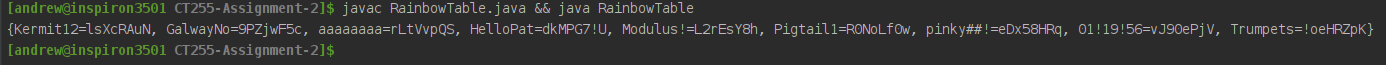
\includegraphics[width = 16cm]{image.png}

\bigskip

%------------------------------------------------

\section{Problem 2}
\subsection{Code}
\begin{lstlisting}[language=java]
import java.util.HashMap;

/*  CT255 Assignment 2
 *  This class provides functionality to build rainbow tables (with a different reduction function per round) for 8 character long strings, which
    consist of the symbols "a .. z", "A .. Z", "0 .. 9", "!" and "#" (64 symbols in total).
    Properly used, it creates the following value pairs (start value - end value) after 10,000 iterations of hashFunction() and reductionFunction():
          start value  -  end value
          Kermit12        lsXcRAuN
          Modulus!        L2rEsY8h
          Pigtail1        R0NoLf0w
          GalwayNo        9PZjwF5c
          Trumpets        !oeHRZpK
          HelloPat        dkMPG7!U
          pinky##!        eDx58HRq
          01!19!56        vJ90ePjV
          aaaaaaaa        rLtVvpQS
          aaaaaaaa        klQ6IeQJ
          
          
 *
 * @author Michael Schukat
 * @version 1.0
 */
public class RainbowTable
{
    public static void main(String[] args) {
		long res = 0;

        // String array of the known passwords
        String[] passwords = {"Kermit12", "Modulus!", "Pigtail1", "GalwayNo", "Trumpets", "HelloPat", "pinky##!", "01!19!56", "aaaaaaaa", "aaaaaaaa"};

        HashMap<String, String> rainbowTable = new HashMap<>(); // declaring a HashTable that i'll use to store the password : hash pairs


        // looping through the passwords array
		for (String start : passwords) {
            if (start.length() != 8) {
                System.out.println("Input " + start + " must be 8 characters long - Exit");
            }
            else {
                String hash = start;                             // declaring a String hash that will hold the final reduced hash of a given password

                // hashing & reducing the start String 10000 times.
                for (int i = 0; i < 10000; i++) {
                    hash = reductionFunction((hashFunction(hash)), i);
                }

                // adding the password & its hash value to the rainbowTable HashMap
                rainbowTable.put(start, hash);
            }
        }
        // printing out the contents of the rainbowTable
        System.out.println(rainbowTable);

        // chain lookup section
        // long array of the 4 hashes to be searched for
        long[] hashes = {895210601874431214L, 750105908431234638L, 111111111115664932L, 977984261343652499L};

        // for each loop that loops through each hash in the array of hashes
        for (long hash : hashes) {

            // looping 10000 times to search for the password - this will function as our max number of iterations, as 10000 iterations should just take use back to where we started.
            for (int i = 0; i < 10000; i++) {
                // reducing the hash
                String str = reductionFunction(hash, i);
                // checking if the reduced hash is a key (password) in the rainbowTable HashMap
                if (rainbowTable.containsValue(str)) {
                    System.out.println("Found password " + str + " for hash value " +  hash);   // printing the found password
                    break;                                                                      // breaking out of the for loop
                }
                else {
                    hash = hashFunction(str);                                                   // hashing str before continuing the for loop
                }
            }
        }
	}
        
    private static long hashFunction(String s){
        long ret = 0;
        int i;
        long[] hashA = new long[]{1, 1, 1, 1};
        
        String filler, sIn;
        
        int DIV = 65536;
        
        filler = new String("ABCDEFGHABCDEFGHABCDEFGHABCDEFGHABCDEFGHABCDEFGHABCDEFGHABCDEFGH");
        
        sIn = s + filler; // Add characters, now have "<input>HABCDEF..."
        sIn = sIn.substring(0, 64); // // Limit string to first 64 characters

        for (i = 0; i < sIn.length(); i++) {
            char byPos = sIn.charAt(i); // get i'th character
            hashA[0] += (byPos * 17111); // Note: A += B means A = A + B
            hashA[1] += (hashA[0] + byPos * 31349);
            hashA[2] += (hashA[1] - byPos * 101302);
            hashA[3] += (byPos * 79001);
        } 
           
        ret = (hashA[0] + hashA[2]) + (hashA[1] * hashA[3]);
        if (ret < 0) ret *= -1;
        return ret;
    } 
    
    private static String reductionFunction(long val, int round) {  // Note that for the first function call "round" has to be 0, 
        String car, out;                                            // and has to be incremented by one with every subsequent call. 
        int i;                                                      // I.e. "round" created variations of the reduction function.
        char dat;                                                  
        
        car = new String("0123456789ABCDEFGHIJKLMNOPQRSTUNVXYZabcdefghijklmnopqrstuvwxyz!#");
        out = new String("");
      
        for (i = 0; i < 8; i++) {
            val -= round;
            dat = (char) (val % 63);
            val = val / 83;
            out = out + car.charAt(dat);
        }
        
        return out;
    }
}

\end{lstlisting}
\subsection{Output}
I couldn't actually find a password match with the above code, and I'm not sure why. My current guess would be that the reduction function wasn't being called properly, as everything else \textit{seemed} to be working as expected. I didn't call the reduction more than 10,000 times as that would theoretically just lead me back to the same place in the chain. I think that my problem is with the passing of the integer \verb|i| to the reduction function, as I think that I correctly implemented the rest of the steps for performing a chain lookup - I input a hash value, reduce it, check if the reduced form is in the list of final plaintexts (the ``Values'' in the HashMap), and if so break out of the loop (but this never occurs), assigning the relevant ``Key'' from the HashMap as the original plaintext password that produced the original input hash. Otherwise, I continue until I'm back at the same place in the chain after the 10,000\textsuperscript{th} iteration, where the code gives up. 

\bigskip

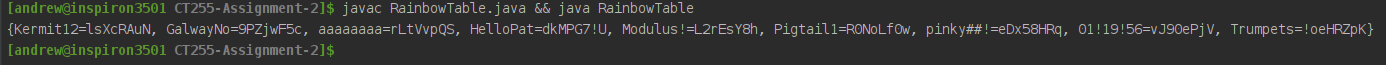
\includegraphics[width = 16cm]{image.png}
\end{document}
